\chapter{Additional timing results}


\begin{figure}[tbph]
    \begin{center}
\begin{tikzpicture}
\begin{axis}[xlabel=Time (seconds), ylabel=Frequency,
grid=major,const plot, ymin=0, enlargelimits=false,
width=12cm, height=5cm, legend style={area legend}]

    \addplot[fill=blue, fill opacity=0.5] table[x=t,y=Text] {gfx/async_text_hist.data};
    
    \addplot[fill=red, fill opacity=0.5] table[x=t,y=Text_c] {gfx/async_text_hist.data};
    
    \addplot+[sharp plot,blue, mark=no marker] coordinates
        {(6.403,0) (6.403,56)};
        
    \addplot+[sharp plot,red, mark=no marker] coordinates
        {(3.463,0) (3.463,56)};
    
    \legend{Cache off,Cache on}
\end{axis}
\end{tikzpicture}

\begin{tikzpicture}
\begin{axis}[xlabel=Time (seconds), ylabel=Frequency,
grid=major,const plot, ymin=0, enlargelimits=false,
width=12cm, height=5cm, legend style={area legend}]
    
    \addplot[fill=blue, fill opacity=0.5] table[x=t,y=Images] {gfx/async_image_hist.data};
    
    \addplot[fill=red, fill opacity=0.5] table[x=t,y=Images_c] {gfx/async_image_hist.data};
    
    \addplot+[sharp plot,blue, mark=no marker] coordinates
        {(19.169,0) (19.169,130)};

    \addplot+[sharp plot,red, mark=no marker] coordinates
        {(4.067,0) (4.067,130)};
    
    \legend{Cache off,Cache on}
    
\end{axis}
\end{tikzpicture}
    \caption{Histogram of 400 page loading times for newsfeeds containing 15 encrypted messages (top) and 15 encrypted images (bottom).}
    \label{graph:hist}
  \end{center}
\end{figure}


\begin{figure}[tbph]
    \begin{center}
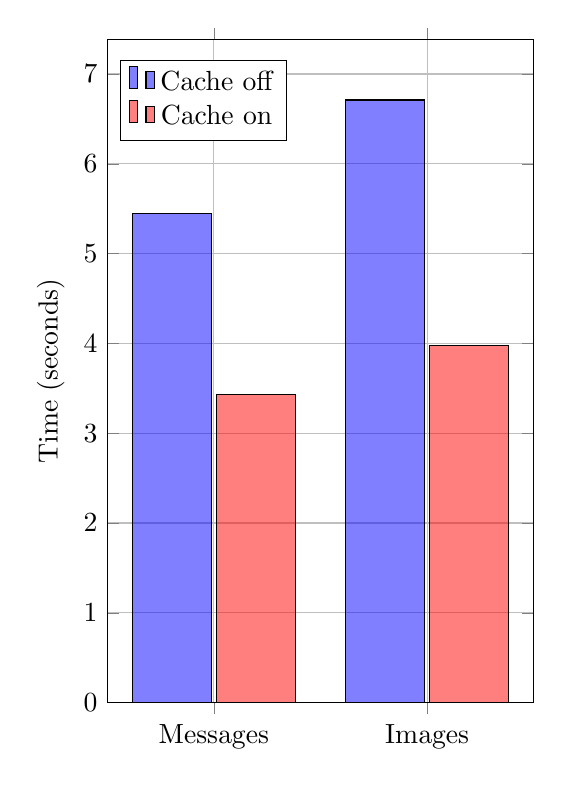
\begin{tikzpicture}
\begin{axis}[grid=major,ybar, 
    symbolic x coords={Messages,Images},
    xtick=data,ylabel=Time (seconds), width=7cm, height=10cm,
    legend style={legend pos=north west, area legend},
    bar width=1cm,enlarge x limits=0.5,ymin=0]
        \addplot[fill=blue, fill opacity=0.5] coordinates { (Messages,5.4457) (Images,6.7105) };
        \addplot[fill=red, fill opacity=0.5] coordinates { (Messages,3.4306) (Images,3.9765) };
        \legend{Cache off, Cache on}
\end{axis}
\end{tikzpicture}
    \caption{Average time before first encrypted item loads.}
    \label{graph:time-first}
  \end{center}
\end{figure}

\begin{figure}
    \begin{center}
        \begin{tikzpicture}
        \begin{axis}[grid=major,ycomb,
        ylabel=Time (ms), 
        width=12cm, height=5cm,
        bar width=0.3cm, ymin=0, xmin=2, xmax=15, enlarge x limits=0.04]
            \addplot[blue] table[x=Item,y=Text] {gfx/async.data};
        \end{axis}
        \end{tikzpicture}
        \begin{tikzpicture}
        \begin{axis}[grid=major,ycomb,
        ylabel=Time (ms), xlabel=Message,
        width=12cm, height=5cm,
        bar width=0.3cm, ymin=0, xmin=2, xmax=15, enlarge x limits=0.04]
            \addplot[red] table[x=Item,y=Text_c] {gfx/async.data};
        \end{axis}
        \end{tikzpicture}
    \caption{Average time interval between successive message loads, with caching turned off and on (top and bottom respectively).}
    \label{graph:txt-rest}
    \end{center}
\end{figure}

\begin{figure}[tbph]
\begin{center}
    
\begin{tikzpicture}
\begin{axis}[grid=major,ycomb,
ylabel=Time (ms), 
width=12cm, height=5cm,
bar width=0.3cm, ymin=0, xmin=2, xmax=15, enlarge x limits=0.04]
    \addplot[blue] table[x=Item,y=Image] {gfx/async.data};
\end{axis}
\end{tikzpicture}

\begin{tikzpicture}
\begin{axis}[grid=major,ycomb,
ylabel=Time (ms),xlabel=Image,
width=12cm, height=5cm,
bar width=0.3cm, ymin=0, xmin=2, xmax=15, enlarge x limits=0.04]
    \addplot[red,] table[x=Item,y=Image_c] {gfx/async.data};
\end{axis}
\end{tikzpicture}

\caption{Average time interval between successive image loads, with caching turned off and on (top and bottom respectively).}
\label{graph:img-rest}
\end{center}
\end{figure}



